% Borg GPU — ORConf 2026 Talk (10 min)
\documentclass[aspectratio=169]{beamer}

% ── No nav clutter for a short talk ─────────────────────────────────────────
\setbeamertemplate{navigation symbols}{}
\setbeamertemplate{footline}[frame number]
\setbeamertemplate{headline}{}

% ── Packages ───────────────────────────────────────────────────────────────
\usepackage[utf8]{inputenc}
\usepackage[T1]{fontenc}
\usepackage{lmodern}
\usepackage{booktabs}
\usepackage{graphicx}
\usepackage{tikz}
\usepackage{xcolor}
\usepackage{enumitem}
\usepackage{url}
\usepackage[final]{qrcode}

% ── Same teal palette as the HPG poster (docs/poster/poster.tex) ───────────
\definecolor{borgblue}{HTML}{085868}
\definecolor{borgorange}{HTML}{E87722}
\definecolor{borggreen}{HTML}{1A9080}
\setbeamercolor{title}{fg=borgblue}
\setbeamercolor{frametitle}{fg=white,bg=borgblue}
\setbeamercolor{structure}{fg=borgblue}
\newcommand{\done}{\textcolor{borggreen}{$\checkmark$}}
\newcommand{\inprog}{{\textcolor{borgblue}{\textbf{[wip]}}}}

\title{Borg}
\subtitle{An Open-Source GPU, Taped Out End-to-End on Libre Silicon Tools}
\author{Andreas Wendleder}
\institute{Independent Researcher \\ \texttt{github.com/gonsolo/Borg}}
\date{ORConf 2026}

\begin{document}

% ── 1: Title ─────────────────────────────────────────────────────────────
\begin{frame}
  \titlepage
\end{frame}

% ── 2: What is Borg (brief — this crowd cares about the toolchain, not the ── %
%      rasterizer) ─────────────────────────────────────────────────────── %
\begin{frame}{What is Borg?}
  \begin{itemize}[leftmargin=*]
    \item A small RISC-V SoC (\textbf{Hutt} core) driving a tile-based
          \textbf{FP16 GPU} as an MMIO peripheral
    \item Chisel HDL, $\sim$19k lines; GPU pipeline itself is $\sim$5.5k LoC
    \item Runs today on a \$100 ECP5 FPGA, HDMI out, real Vulkan content
          via a native Mesa ICD (\texttt{borgvk})
  \end{itemize}
  \vfill
  \centering
  \textcolor{borgorange}{\textbf{But that's not really the point of this talk.}}
\end{frame}

% ── 3: Reframe — the real story is the toolchain ────────────────────────── %
\begin{frame}{Why This Talk is Here, Not at a Graphics Conference}
  \begin{itemize}[leftmargin=*]
    \item Borg has already been presented as a GPU (HPG 2026)
    \item Here, Borg is a \textbf{stress test}: is a fully libre EDA flow
          capable of taking a non-trivial SoC —
          RISC-V core \emph{and} a custom floating-point pipeline —
          all the way to \textbf{signed-off silicon}?
    \item To our knowledge: the first open-source GPU with a
          \textbf{submitted ASIC tapeout}
  \end{itemize}
\end{frame}

% ── 4: Toolchain ─────────────────────────────────────────────────────────
\begin{frame}{The Toolchain: Zero Proprietary Tools}
  \centering
  \begin{tabular}{@{}ll@{}}
    \textbf{HDL}         & Chisel (Scala) \\
    \textbf{Synthesis}   & Yosys \\
    \textbf{P\&R / Signoff} & \textbf{LibreLane} (OpenROAD, Magic, KLayout, Netgen) \\
    \textbf{Simulation}  & Verilator, cocotb, Arcilator \\
    \textbf{Reg.\ map}   & SystemRDL $\to$ PeakRDL-chisel \\
    \textbf{PDKs}        & IHP SG13G2, GF180MCU \\
    \textbf{Environment} & Nix flakes — one \texttt{nix develop}, zero manual installs
  \end{tabular}
  \vfill
  \centering
  \textcolor{borgorange}{\textbf{Reproducibility as a first-class design goal,}}\\
  \textcolor{borgorange}{\textbf{not an afterthought.}}
\end{frame}

% ── 5: Tapeouts ──────────────────────────────────────────────────────────
\begin{frame}{Two Tapeouts in Flight}
  \centering \small
  \begin{tabular}{@{}llll@{}}
    \toprule
    \textbf{Shuttle} & \textbf{PDK} & \textbf{Flow} & \textbf{Status} \\
    \midrule
    Tiny Tapeout (TTIHP26a) & IHP SG13G2 (130\,nm) & LibreLane & Submitted; chips $\approx$ Sept.\ 2026 \\
    wafer.space             & GF180MCU             & LibreLane & In signoff \\
    \bottomrule
  \end{tabular}
  \vfill
  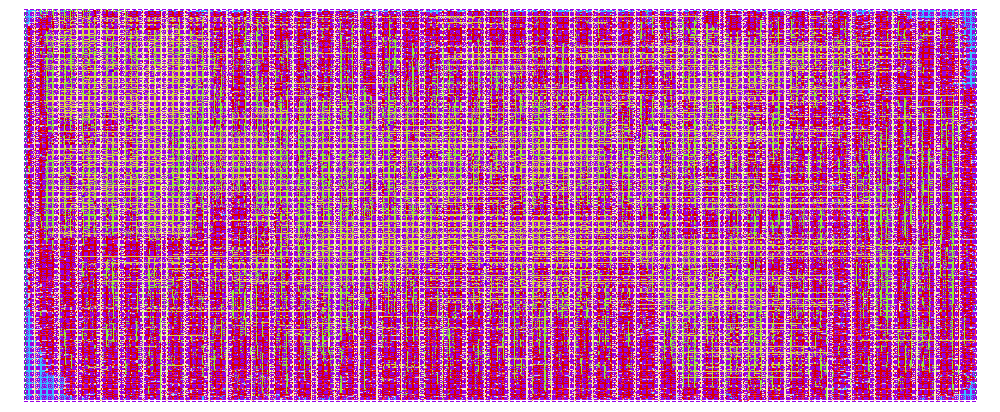
\includegraphics[width=0.32\linewidth]{../poster/gds_render_small}
\end{frame}

% ── 6: War stories — THE payload for this audience ──────────────────────── %
\begin{frame}{What Breaks When You Actually Push These Tools to Tapeout}
  \begin{itemize}[leftmargin=*]
    \item \textbf{Yosys}: \texttt{autoname} pass rescans the whole module
          every iteration — $O(n^2)$ blowup, 49\,GB+/never-complete on our
          SoC. Patched locally, fixed upstream (yosys \#6050) and shipped
          in \texttt{0.68}, our current pin — local patch dropped.
    \item \textbf{LibreLane 3.0.3 \texttt{--manual-pdk}}: three real signoff
          blockers (dead VDD/DVDD tie, unset \texttt{DEFAULT\_CORNER},
          a PDN config hardcoding macros we don't have). Fixed upstream,
          now on \texttt{3.0.8}.
    \item \textbf{OpenROAD}: a heap-underflow crash (\texttt{GRT-0183})
          during antenna-repair jumper insertion, hit on a real net in our
          own GDS flow — already fixed upstream, pulled in via our own
          nixpkgs 26Q2$\to$26Q3 OpenROAD bump.
    \item \textbf{KLayout DRC}: \texttt{0.30.10}'s \texttt{separation()}
          operator spuriously flagged fully-overlapping regions as a
          sealring DRC violation (\texttt{GR.2}) — a regression, not a
          real bug, confirmed against the PDK's own unmodified code.
          Fixed upstream (\#2425), adopted in \texttt{0.30.11}.
  \end{itemize}
  \vfill
  \centering
  \textcolor{borgorange}{\textbf{Every one of these was reported, and where}}\\
  \textcolor{borgorange}{\textbf{possible fixed, upstream — not worked around silently.}}
\end{frame}

% ── 6b: The Bluespec detour — a different kind of tool story ─────────────
\begin{frame}{When Chisel (and an LLM) Got Stuck: A Bluespec Detour}
  \begin{itemize}[leftmargin=*]
    \item A race condition in the memory controller's QSPI bus arbiter
          resisted both manual debugging \emph{and} LLM-assisted fixes
          in Chisel/simulation
    \item Ported the $\sim$3-class arbitration logic to \textbf{Bluespec
          SystemVerilog} — a different open HDL, built around
          \emph{atomic rule scheduling} with static conflict checking
    \item Bluespec's compiler resolved the correct priority chain
          (\texttt{CPU Read > CPU Write > GPU Write > GPU Read > Instr
          Fetch} via \texttt{descending\_urgency}) in a fraction of a
          second
    \item Ported the verified logic back into Chisel by hand
  \end{itemize}
  \vfill
  \centering
  \textcolor{borgorange}{\textbf{Different HDL semantics catch different}}\\
  \textcolor{borgorange}{\textbf{bug classes — worth more than one tool in the box.}}
\end{frame}

% ── 7: Ecosystem contribution ────────────────────────────────────────────
\begin{frame}{A Year of Upstream Maintenance}
  \centering
  {\Large \textbf{80+ contributions}, July 2025 -- July 2026}
  \vspace{0.8em}

  \small
  \begin{tabular}{@{}lr@{}}
    \toprule
    \textbf{Target} & \textbf{Merged PRs} \\
    \midrule
    \texttt{nixpkgs} & 51 \\
    \texttt{librelane/librelane} & 5 \\
    OpenROAD, PeakRDL, Chisel, rocket-chip, riscv-boom, tt-support-tools & 8 \\
    AUR (Arch) packages & 5+ \\
    \bottomrule
  \end{tabular}

  \vspace{1em}
  \raggedright \normalsize
  \textbf{Packages authored from scratch} for \texttt{nixpkgs}: \\
  \texttt{librelane}, \texttt{netgen-vlsi}, \texttt{riscv-model},
  \texttt{pdk-ciel}, \texttt{libparse-python}, \texttt{gdstk} — plus
  several more on AUR.
\end{frame}

% ── 7b: Why it matters ────────────────────────────────────────────────────
\begin{frame}{Why Package the Tools, Not Just Use Them}
  \begin{itemize}[leftmargin=*]
    \item \textbf{LibreLane itself} — the tool most of this flow (and much
          of this room) depends on — reached \texttt{nixpkgs} through this
          project
    \item Whole flow is one \texttt{flake.nix}: same bits, same bugs,
          same fixes, for anyone who clones the repo
    \item Packaging surfaces bugs that using-in-place never would —
          reproducible builds are also a debugging tool
  \end{itemize}
\end{frame}

% ── 8: Funding & status ──────────────────────────────────────────────────
\begin{frame}{Funding \& Status}
  \centering
  
\includegraphics[height=1.6cm]{../poster/figures/nlnet_logo}
  \qquad
  
\includegraphics[height=1.6cm]{../poster/figures/ngi0_logo}
  \vspace{1em}

  \small
  Funded by the \textbf{NGI0 Commons Fund} (NLnet / European Commission,
  Grant No.~101135429) and Swiss SERI.

  \vspace{1em}
  \begin{itemize}[leftmargin=*]
    \item Phase 1--3 \done\ (architecture, autonomy, HPG demo)
    \item Phase 4--5, 7 \inprog\ (Linux-capable CPU, Mesa Vulkan driver,
          Vulkan 1.0 conformance)
  \end{itemize}
\end{frame}

% ── 9: Call to action ─────────────────────────────────────────────────────
\begin{frame}{Get Involved}
  \begin{itemize}[leftmargin=*]
    \item Everything is open: RTL, compiler, firmware, GDS, the Nix flake
          itself
    \item Looking for: EDA toolchain reviewers, PDK/DRC eyes, anyone who
          wants to reproduce the tapeout flow end-to-end
  \end{itemize}
  \vfill
  \begin{center}
    \begin{minipage}{0.45\linewidth}
      \centering
      \qrcode[height=2.6cm]{https://github.com/gonsolo/Borg}\\[0.2em]
      {\small\textbf{Source Code}}
    \end{minipage}
    \hfill
    \begin{minipage}{0.45\linewidth}
      \centering
      \qrcode[height=2.6cm]{https://gonsolo.github.io/Borg}\\[0.2em]
      {\small\textbf{Book / Docs}}
    \end{minipage}
  \end{center}
\end{frame}

% ── 10: Thanks ────────────────────────────────────────────────────────────
\begin{frame}
  \centering
  {\LARGE Thank you}
  \vspace{1em}

  \texttt{andreas.wendleder@proton.me}\\
  \texttt{github.com/gonsolo/Borg}
\end{frame}

\end{document}
